\subsubsection{Set 3 - Greenyard Maaseik}
\label{sec:PL3_Greenyard3}
%TODO: tekst aanpassen
Bij de opslag komt het teken \# overeen met 0, + en / met 1, ! met 2, - en = met 3.

In figuur \ref{fig:PL3ServeMaaseik3} zijn de receptie- en opslagstatistieken weergegeven. Hier zijn het totaal aantal opslagen én perfecte opslagen gelijk. Bij de andere scores zijn de opslagen ongeveer gelijk verdeeld.

De beoordeling van de receptie is op een andere wijze gedaan dan bij de manuele invoer. Bij de manuele invoer wordt er gebruik gemaakt van tekens, terwijl bij de AI-invoer gebruik wordt gemaakt van cijfers. Bij de receptie komt het teken \# overeen met 3, + en / met 2, ! met 1, - en = met 0.

Bij deze statistieken kan geconstateerd worden dat de AI-invoer bepaalde spelers niet heeft geregisteerd. Aan één speler heeft de AI ook een receptie meer gegeven dan de manuele invoer. Opmerkelijk is wel dat de manuele invoer hier voor bepaalde recepties positiever is. Er zijn meer opslagen met een score 3 bij de manuele invoer dan bij de AI.

\begin{figure}[ht]
\centering
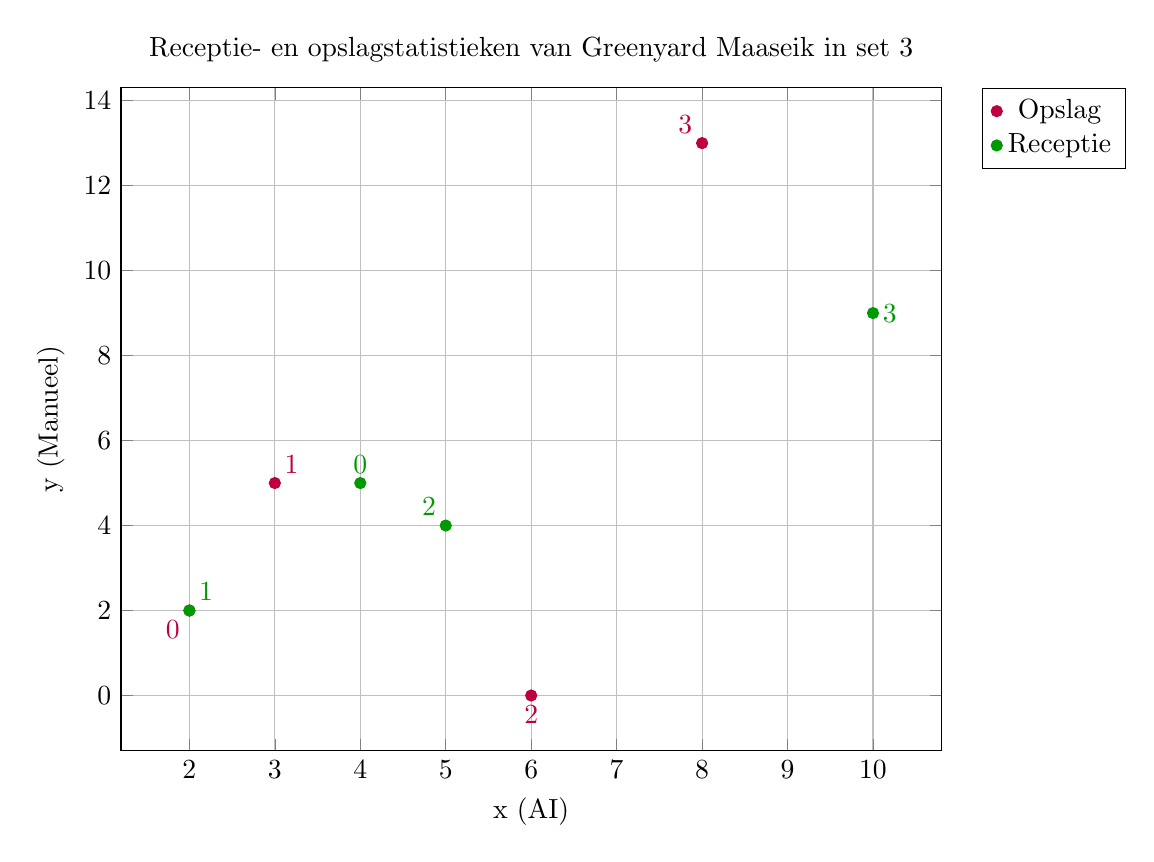
\begin{tikzpicture}
  \begin{axis}[
    title={Receptie- en opslagstatistieken van Greenyard Maaseik in set 3},
    xlabel={x (AI)},
    ylabel={y (Manueel)},
    grid=major,
    legend style={at={(1.05,1)}, anchor=north west},
    width=12cm,
    height=10cm,
    enlargelimits=0.1,
  ]

  % Opslag
  \addplot[
    only marks,
    mark=*,
    color=purple,
  ] table {
    x y
    2 2
    3 5
    6 0
    8 13
  };
  \addlegendentry{Opslag}

  % Labels opslag
  \node at (axis cs:2,2) [anchor=north east, purple] {0};
  \node at (axis cs:3,5) [anchor=south west, purple] {1};
  \node at (axis cs:6,0) [anchor=north, purple] {2};
  \node at (axis cs:8,13) [anchor=south east, purple] {3};

  % Receptie
  \addplot[
    only marks,
    mark=*,
    color=green!60!black,
  ] table {
    x y
    10 9
    5 4
    2 2
    4 5
  };
  \addlegendentry{Receptie}

  % Labels receptie
  \node at (axis cs:10,9) [anchor=west, green!60!black] {3};
  \node at (axis cs:5,4) [anchor=south east, green!60!black] {2};
  \node at (axis cs:2,2) [anchor=south west, green!60!black] {1};
  \node at (axis cs:4,5) [anchor=south, green!60!black] {0};

  \end{axis}
\end{tikzpicture}
\caption{AI invoer versus manuele invoer, ingedeeld in opslag en receptie, voor Greenyard Maaseik in set 3.}
\label{fig:PL3ServeMaaseik3}
\end{figure}

De spelverdelingsstatistieken zijn te vinden in tabel \ref{tab:PL3SetMaaseikMan3} en \ref{tab:PL3SetDigMaaseikAI3}. Die van de verdeding zijn dan weer te vinden in tabel \ref{tab:PL3DigMaaseikMan3} en \ref{tab:PL3SetDigMaaseikAI3}. 

Enkel één speler heeft een verschillend totaal aantal spelverdedingsacties. Bij de manuele invoer heeft hij er géén gedaan, terwijl hij er bij de AI-invoer één heeft gedaan. 

Bij de verdedigingsstatistieken ontbreken er bij de AI-invoer enkele spelers of hebben ze minder ondernomen. 

\begin{table}[ht!]
    \centering
    \scriptsize
    \begin{tabular}{|l|c|c|c|c|c|c|c|c|c|} \hline
        \textbf{Speler} & *E\% & Tot & = & / & - & ! & + & \#\\ \hline
        Renet Vancker & 100\% & 3 &  &  &  &  & 2 & 1 \\ 
        Dawid Pawlun & 100\% & 17 &  &  &  &  & 15 & 2 \\ 
        Pierre Perin & 100\% & 2 &  &  &  &  & 2 &  \\ \hline
    \end{tabular}
    \caption[Manueel ingevoerde spelverdelingsstatistieken voor Greenyard Maaseik in set 3]{\label{tab:PL3SetMaaseikMan3}Manueel ingevoerde spelverdelingsstatistieken voor Greenyard Maaseik in set 3.}
\end{table}

\begin{table}[ht!]
    \centering
    \scriptsize
    \begin{tabular}{|l|c|c|c|c|c|c|c|c|c|} \hline
        \textbf{Speler} & *E\% & Tot & = & / & - & ! & + & \#\\ \hline
        Samuel Fafchamps & 0\% & 1 & 1 &  &  &  &  &  \\ 
        Jolan Cox & 50\% & 2 & 1 & 1 &  &  &  & \\
        Landon Douglas Currie & 33\% & 3 & 1 &  & 1 &  & 1 &  \\
        Dawid Pawlun & 0\% & 3 & 2 &  & 1 &  &  &  \\ 
        Hampus Ekstrand & 100\% & 1 &  &  &  &  & 1 &\\ 
        Pierre Perin & 100\% & 1 &  &  &  &  & 1 & \\ \hline
    \end{tabular}
    \caption[Manueel ingevoerde verdedigingsstatistieken voor Greenyard Maaseik in set 3]{\label{tab:PL3DigMaaseikMan3}Manueel ingevoerde verdedigingsstatistieken voor Greenyard Maaseik in set 3.}
\end{table}

\begin{table}[ht!]
  \centering
  \scriptsize
    \begin{tabular}{|l|c|c|c|c|c|c|c|} \hline
    \textbf{Speler} & Ast & TA & SE & PCT & DS & DE \\ \hline
    Renet Vancker & 2 & 3 &  & 67\% &   &   \\
    Landon Douglas Currie &  & 1 &  & 0\% & 2 & 1 \\
    Dawid Pawlun & 8 & 17 & & 47\% & 2 &  \\
    Hampus Ekstrand &  &  &  &  & 3 &  \\
    Pierre Perin &  & 2 &  & 0\% & 1 &  \\ \hline
  \end{tabular}
  \caption[Spelverdelings- en verdedigingsstatistieken gemaakt door Balltime AI voor Greenyard Maaseik in set 3]{\label{tab:PL3SetDigMaaseikAI3}Spelverdelings- en verdedigingsstatistieken gemaakt door Balltime AI voor Greenyard Maaseik in set 3.}
\end{table}

In tabellen \ref{tab:PL3AttMaaseikMan3} en \ref{tab:PL3BlockMaaseikMan3} zijn de manueel ingevoerde aanvals- en blokstatistieken weergegeven. In tabel \ref{tab:PL3AttBlockMaaseikAI3} zijn de aanvals- en blokstatistieken weergegeven die door Balltime AI zijn gemaakt. 

Het aantal aanvallen is bij beide hetzelfde, behalve bij één speler. Hij heeft een aanval meer bij de AI-invoer. De foutieve aanvallen zijn wel verschillend bij beide. Bij de aanval met de AI-invoer valt op dat Alex Saaremaa een aanval heeft gedaan, wanneer er de beelden worden bekeken is er eigenlijk geen aanval te zien. De AI dacht dat hij een aanval deed, maar eigenlijk is de bal langs hem heen gegaan.

Bij de blokkeringen is er een zeer groot verschil. Bij de AI-invoer zijn er maar twee geweest in de hele set. Terwijl er bij de manuelen invoer dertien blokkeringen zijn geteld.

\begin{table}[ht!]
    \centering
    \scriptsize
    \begin{tabular}{|l|c|c|c|c|c|c|c|c|c|} \hline
        \textbf{Speler} & *E\% & Tot & = & / & - & ! & + & \#\\ \hline
        Samuel Fafchamps & 100\% & 1 &  &  &  &  &  & 1 \\ 
        Jolan Cox & 33\% & 12 &  & 2 &  & 1 & 3 & 6 \\ 
        Miquel Angel Fornés & 33\% & 3 &  & 1 &  &  &  & 2 \\ 
        Hampus Ekstrand & -50\% & 2 & 1 &  &  &  & 1 & \\ 
        Pierre Perin & -50\% & 4 & 3 &  &  &  &  & 1 \\ \hline
    \end{tabular}
    \caption[Manueel ingevoerde aanvalsstatistieken voor Greenyard Maaseik in set 3]{\label{tab:PL3AttMaaseikMan3}Manueel ingevoerde aanvalsstatistieken voor Greenyard Maaseik in set 3.}
\end{table}

\begin{table}[ht!]
    \centering
    \scriptsize
    \begin{tabular}{|l|c|c|c|c|c|c|c|c|c|} \hline
        \textbf{Speler} & *E\% & Tot & = & / & - & ! & + & \#\\ \hline
        Samuel Fafchamps & 33\% & 3 &  &  &  & 1 & 1 & 1 \\ 
        Jolan Cox & -75\% & 4 & 3 &  &  & 1 &  & \\ 
        Dawid Pawlun & -33\% & 3 & 1 &  & 1 & 1 &  &  \\ 
        Miquel Angel Fornés & -100\% & 1 & 1 &  &  &  &  & \\ 
        Hampus Ekstrand & 50\% & 2 &  &  &  & 1 &  & 1 \\  \hline
    \end{tabular}
    \caption[Manueel ingevoerde blokstatistieken voor Greenyard Maaseik in set 3]{\label{tab:PL3BlockMaaseikMan3}Manueel ingevoerde blokstatistieken voor Greenyard Maaseik in set 3.}
\end{table}

\begin{table}[ht!]
  \centering
  \scriptsize
  \begin{tabular}{|l|c|c|c|c|c|c|c|c|c|c|c|} \hline
    \textbf{Speler} & K & E & TA & Atk\% & Kill\% & Error\% & BS & BA & BE \\ \hline
    Samuel Fafchamps & 1 &  & 1 & 1.00 & 100\% & 0\% &  &   &  \\
    Jolan Cox & 6 & 2 & 12 & 0.33 & 50\% & 17\% &  &   &  \\
    Dawid Pawlun &   &   &   &   &   &   & 1 & & \\
    Miquel Angel Fornés & 2 & 1 & 3 & 0.33 & 67\% & 33\% &  &   &  \\
    Hampus Ekstrand &  & 1 & 2 & -0.50 & 0\% & 50\% & 1 & & \\
    Alex Saaremaa &  &  & 1 & 0.00 & 0\% & 0\% &  & &\\
    Pierre Perin & 1 & 3 & 5 & -0.40 & 20\% & 60\% & &  & \\  \hline
  \end{tabular}
  \caption[Aanvals- en blokstatistieken gemaakt door Balltime AI voor Greenyard Maaseik in set 3]{\label{tab:PL3AttBlockMaaseikAI3}Aanvals- en blokstatistieken gemaakt door Balltime AI voor Greenyard Maaseik in set 3.}
\end{table}
